\documentclass[../main.tex]{subfiles}
\begin{document}
\subsection{Motivation}\label{subsec1.1}
As briefly introduced above, critical transitions are often associated to catastrophic and abrupt regime shifts observed in a variety of natural and human complex systems.
As the system evolves by (slowly) tracking a stable equilibrium a sudden and often unforeseen change in the dynamics brings the state observables to be repelled away from the attractor in a rapid fashion. The state becomes unstable and it evolves much more quickly with respect to (w.r.t.) the timescale that characterised its dynamics prior to the regime shift.
Despite the rather severe tone, these type of events appear to be ubiquitous in complex systems. 
One classical example is given by the global tipping points of the Earth's climate \cite{Lenton11} driven by anthropogenic climate change, however paleoclimatic extreme events \cite{Dakos08} s.a. the end of the Greenhouse Earth at around 34 million years ago (Figure \ref{fig1.1}(a)), the end of the last ice age that occured about 10,000 years ago (Figure \ref{fig1.1}(b)) and the most recent end of the African humid period at approximately 3000 BCE (Figure \ref{fig1.1}(c)) all happened without human input.
Similarly to climate critical thresholds, catastrophic regime shifts also appear quite frequently as population collapses of living, interacting organisms observed in natural ecosystems \cite{Scheffer01} as well as in-vitro (Figure \ref{fig1.1}(d)) and in-silico \cite{Carpenter06} lab experiments.
In addition, seemingly unrelated natural sciences s.a. physics, biology and medicine also feature similar tipping points. 
Evidence of abrupt transitions were found recently in magnetic quantum phase transitions (Figure \ref{fig1.1}(e)).
In vital human biological systems some examples are the exacerbation of ventilation defects prior to the onset of asthma \cite{Venegas05}, pre-ictal dynamic changes before epileptic seizures \cite{Litt01,McSharry03}, mood instabilities symptomatic of major depressive disorder (MDD) \cite{Leemput13} (albeit lacking substantial empirical proof \cite{Bos14}) and pathological sleep-quality disruptions \cite{deMooij20}.
Finally human sciences have also started to recently characterise disruptive phenomena as critical transitions with particular emphasis being pursued in real \cite{Scheffer21} and simulated \cite{Suweis14,Liang17} social networks and opinion dynamics \cite{Brock06} as well as in the study of the collapse of financial markets (Figure \ref{fig1.1}(f)) in complex macroeconomic systems \cite{Kozlowska16,Kai20}.
Given this wide and impactful range of different phenomena, the topic of reliably detecting indicators of critical transitions has attracted ever growing attention and in the past two decades several efforts have tried to associate signs of incoming criticalities with measurable quantities as we describe in the next Section.
\begin{figure}[H]
    \centering 
    \begin{subfigure}[b]{0.325\textwidth}
        \centering 
        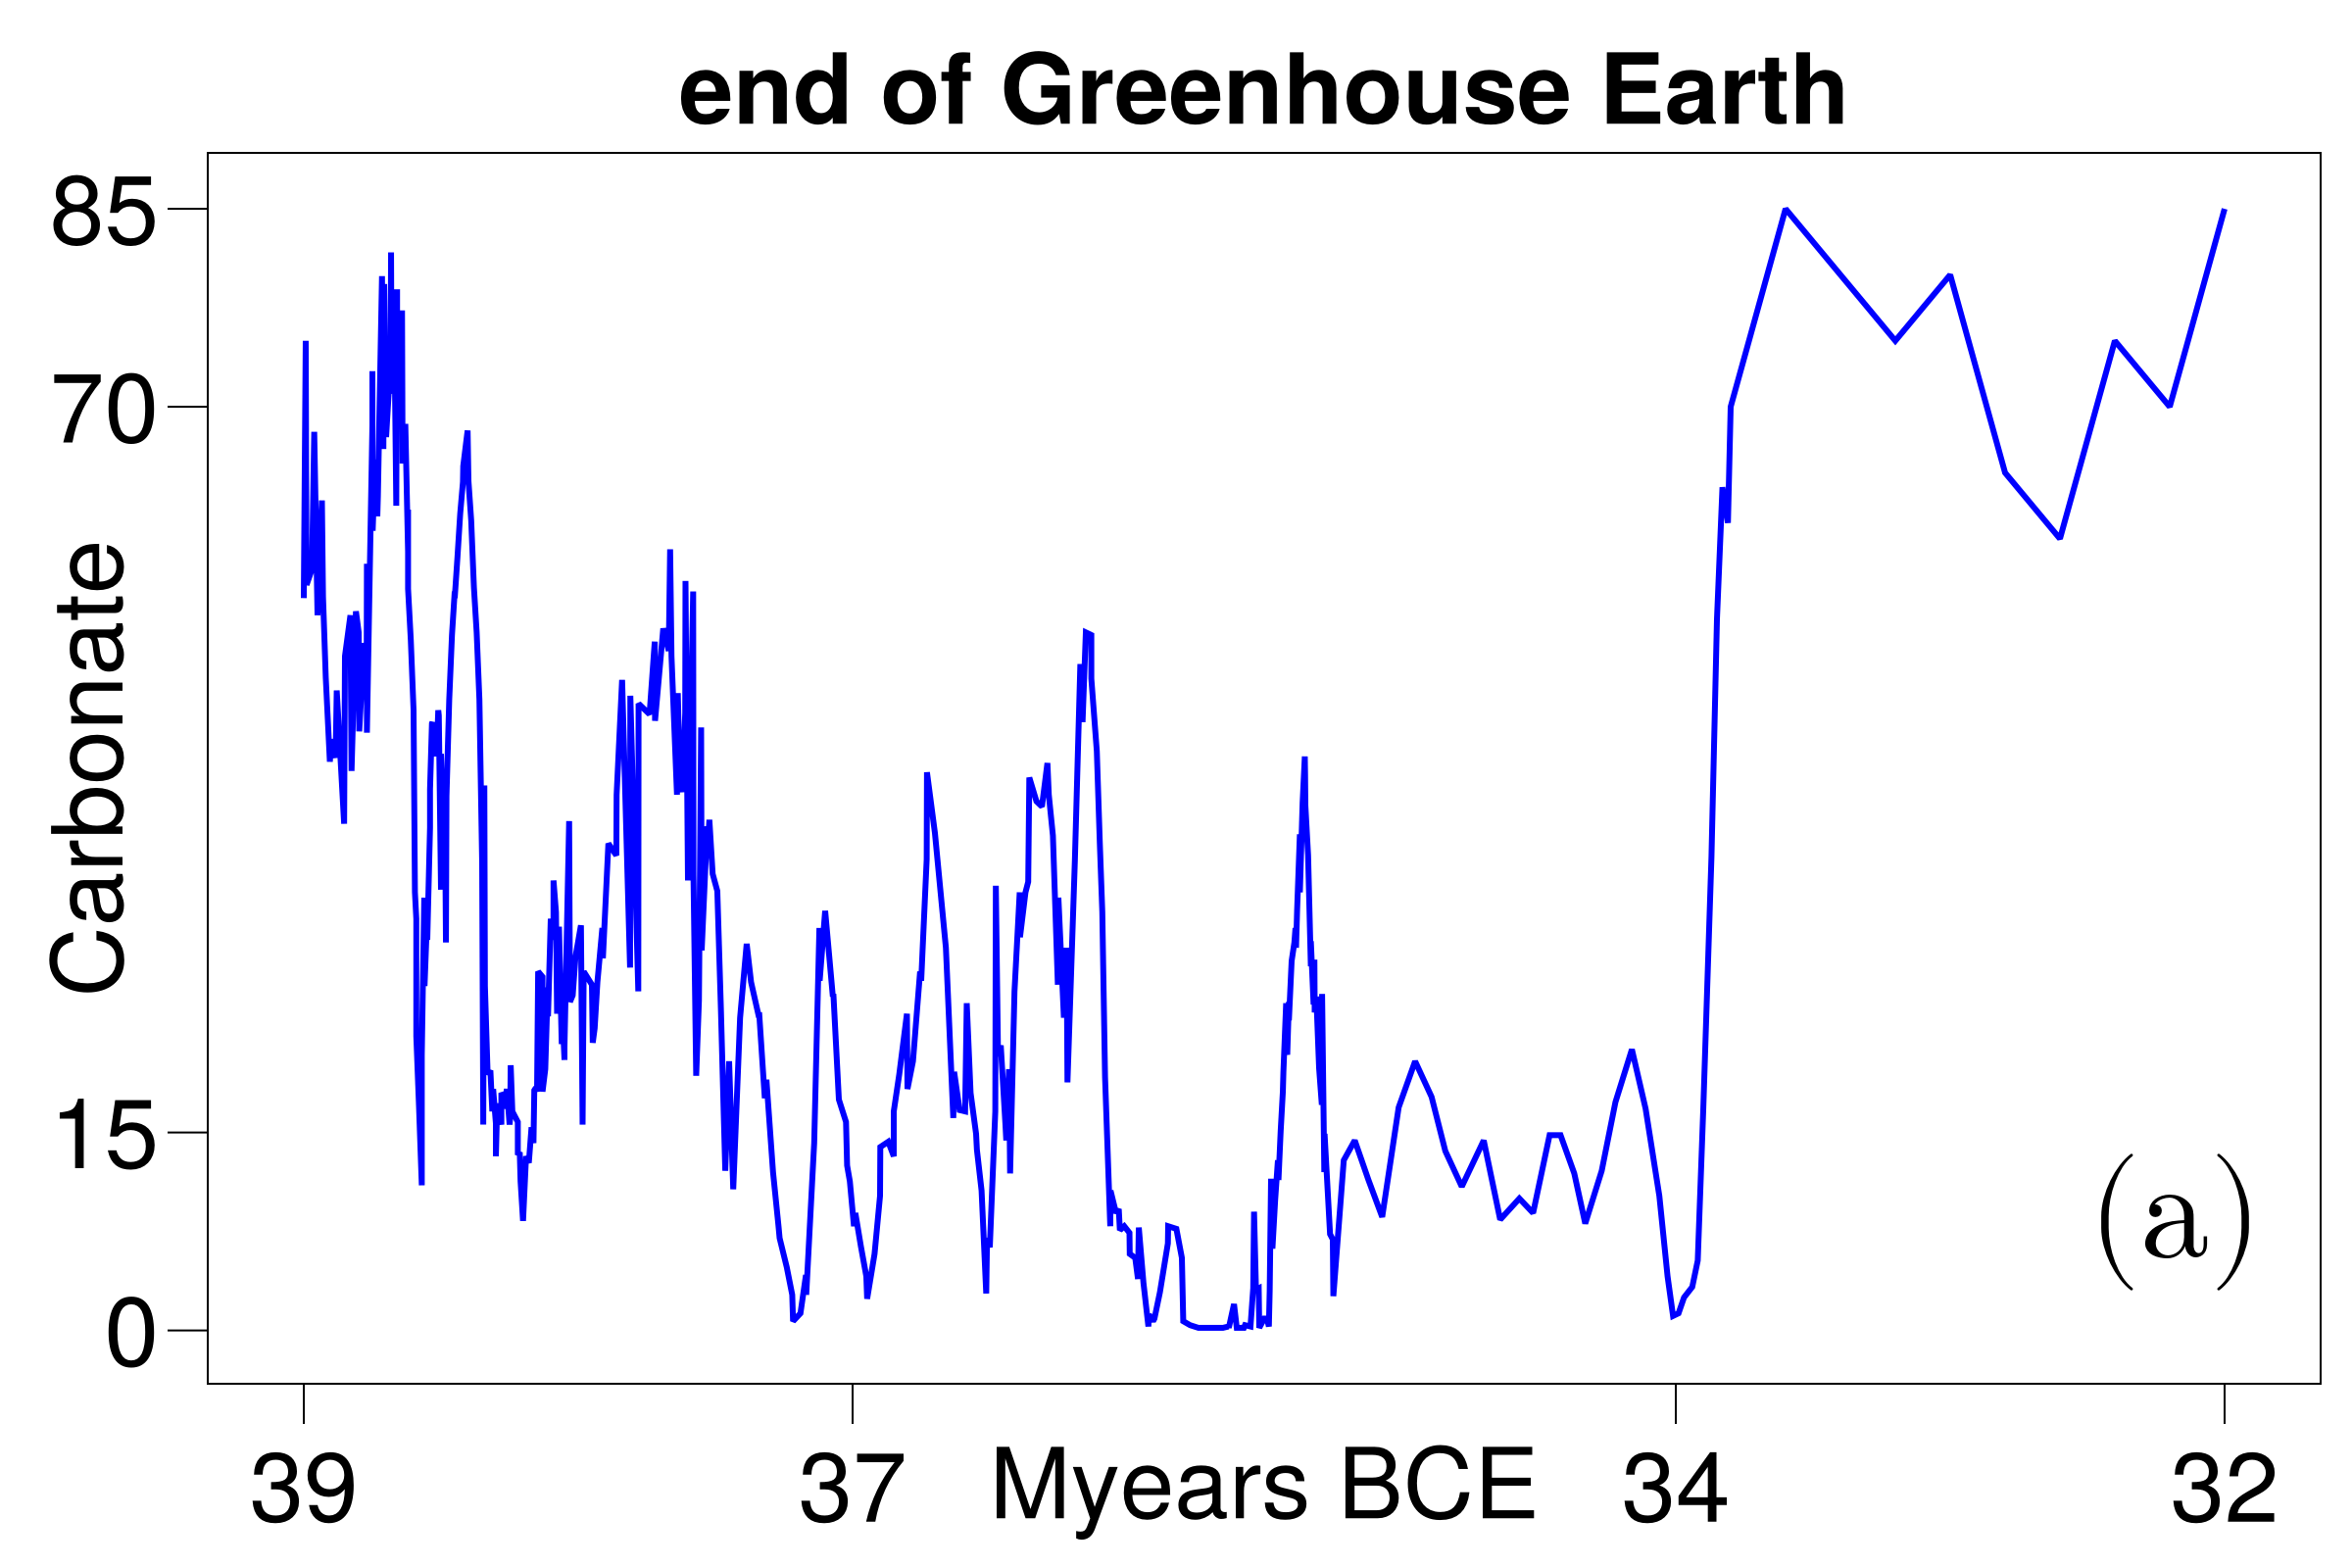
\includegraphics[keepaspectratio, width = \linewidth]{../figures/fig1.1.1.png}
        \label{fig1.1.1}
    \end{subfigure}
    \hfill
    \begin{subfigure}[b]{0.325\textwidth}
        \centering 
        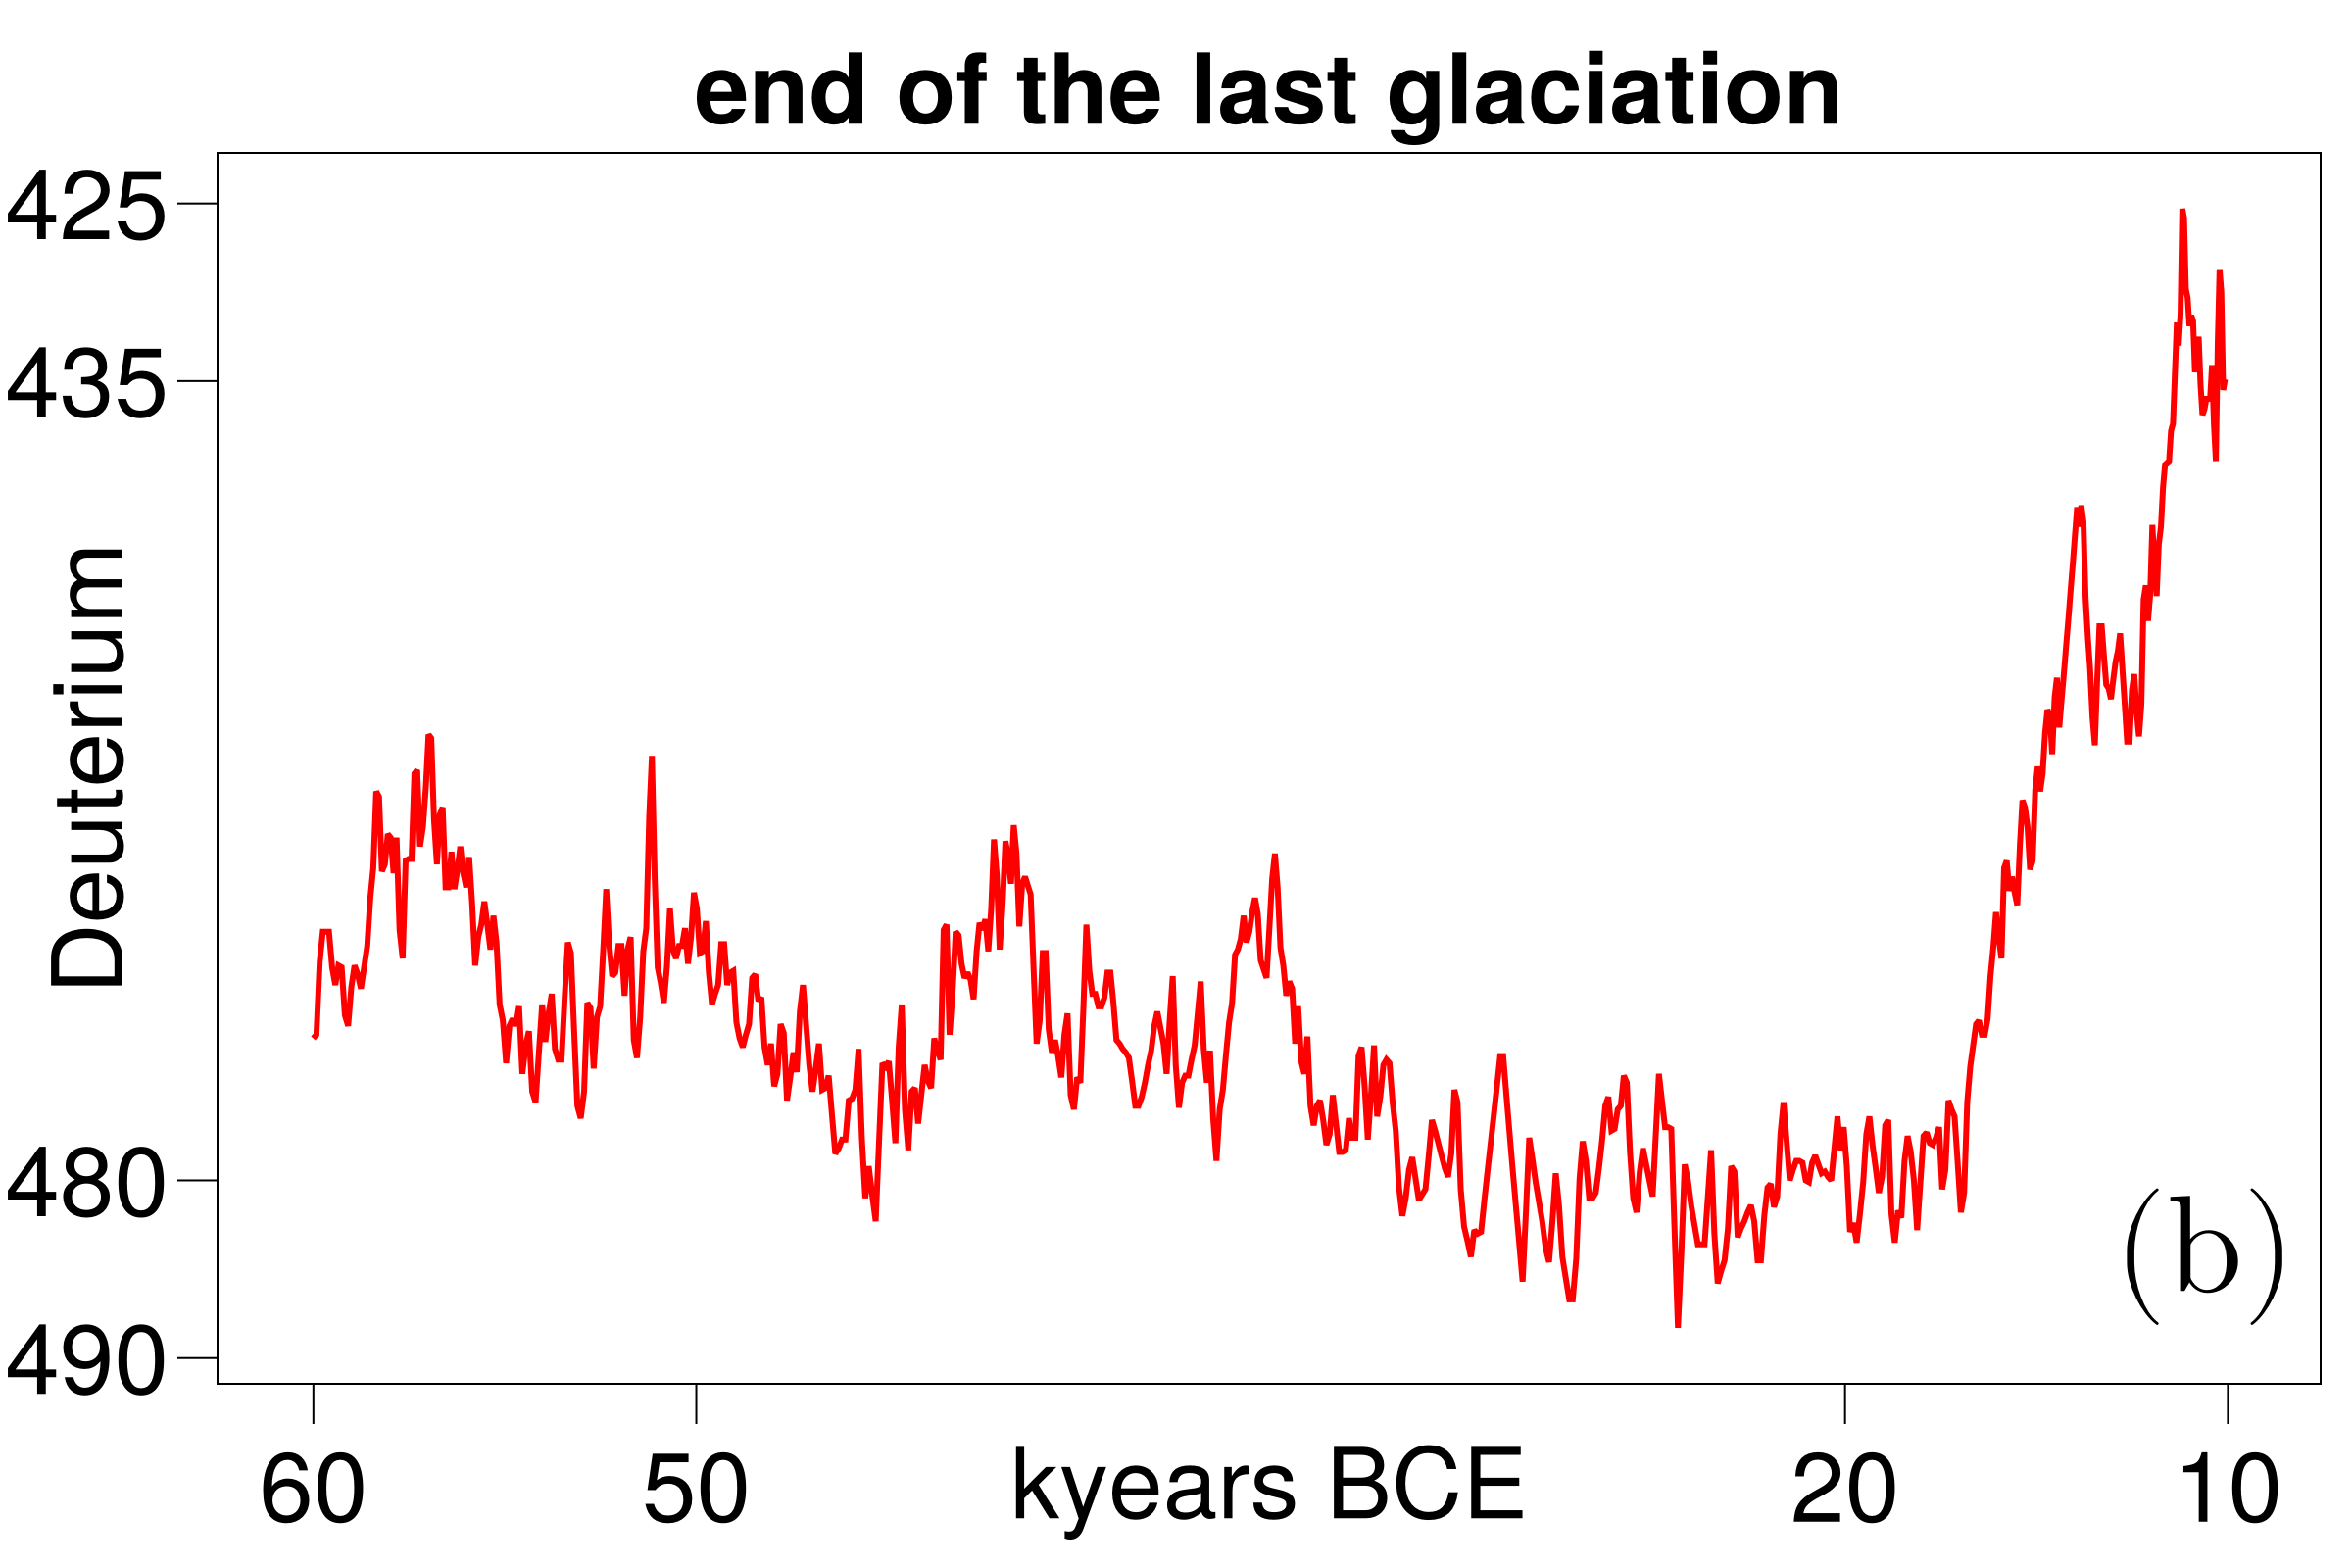
\includegraphics[keepaspectratio, width = \linewidth]{../figures/fig1.1.2.png}
        \label{fig1.1.2}
    \end{subfigure}
    \hfill
    \begin{subfigure}[b]{0.325\textwidth}
        \centering 
        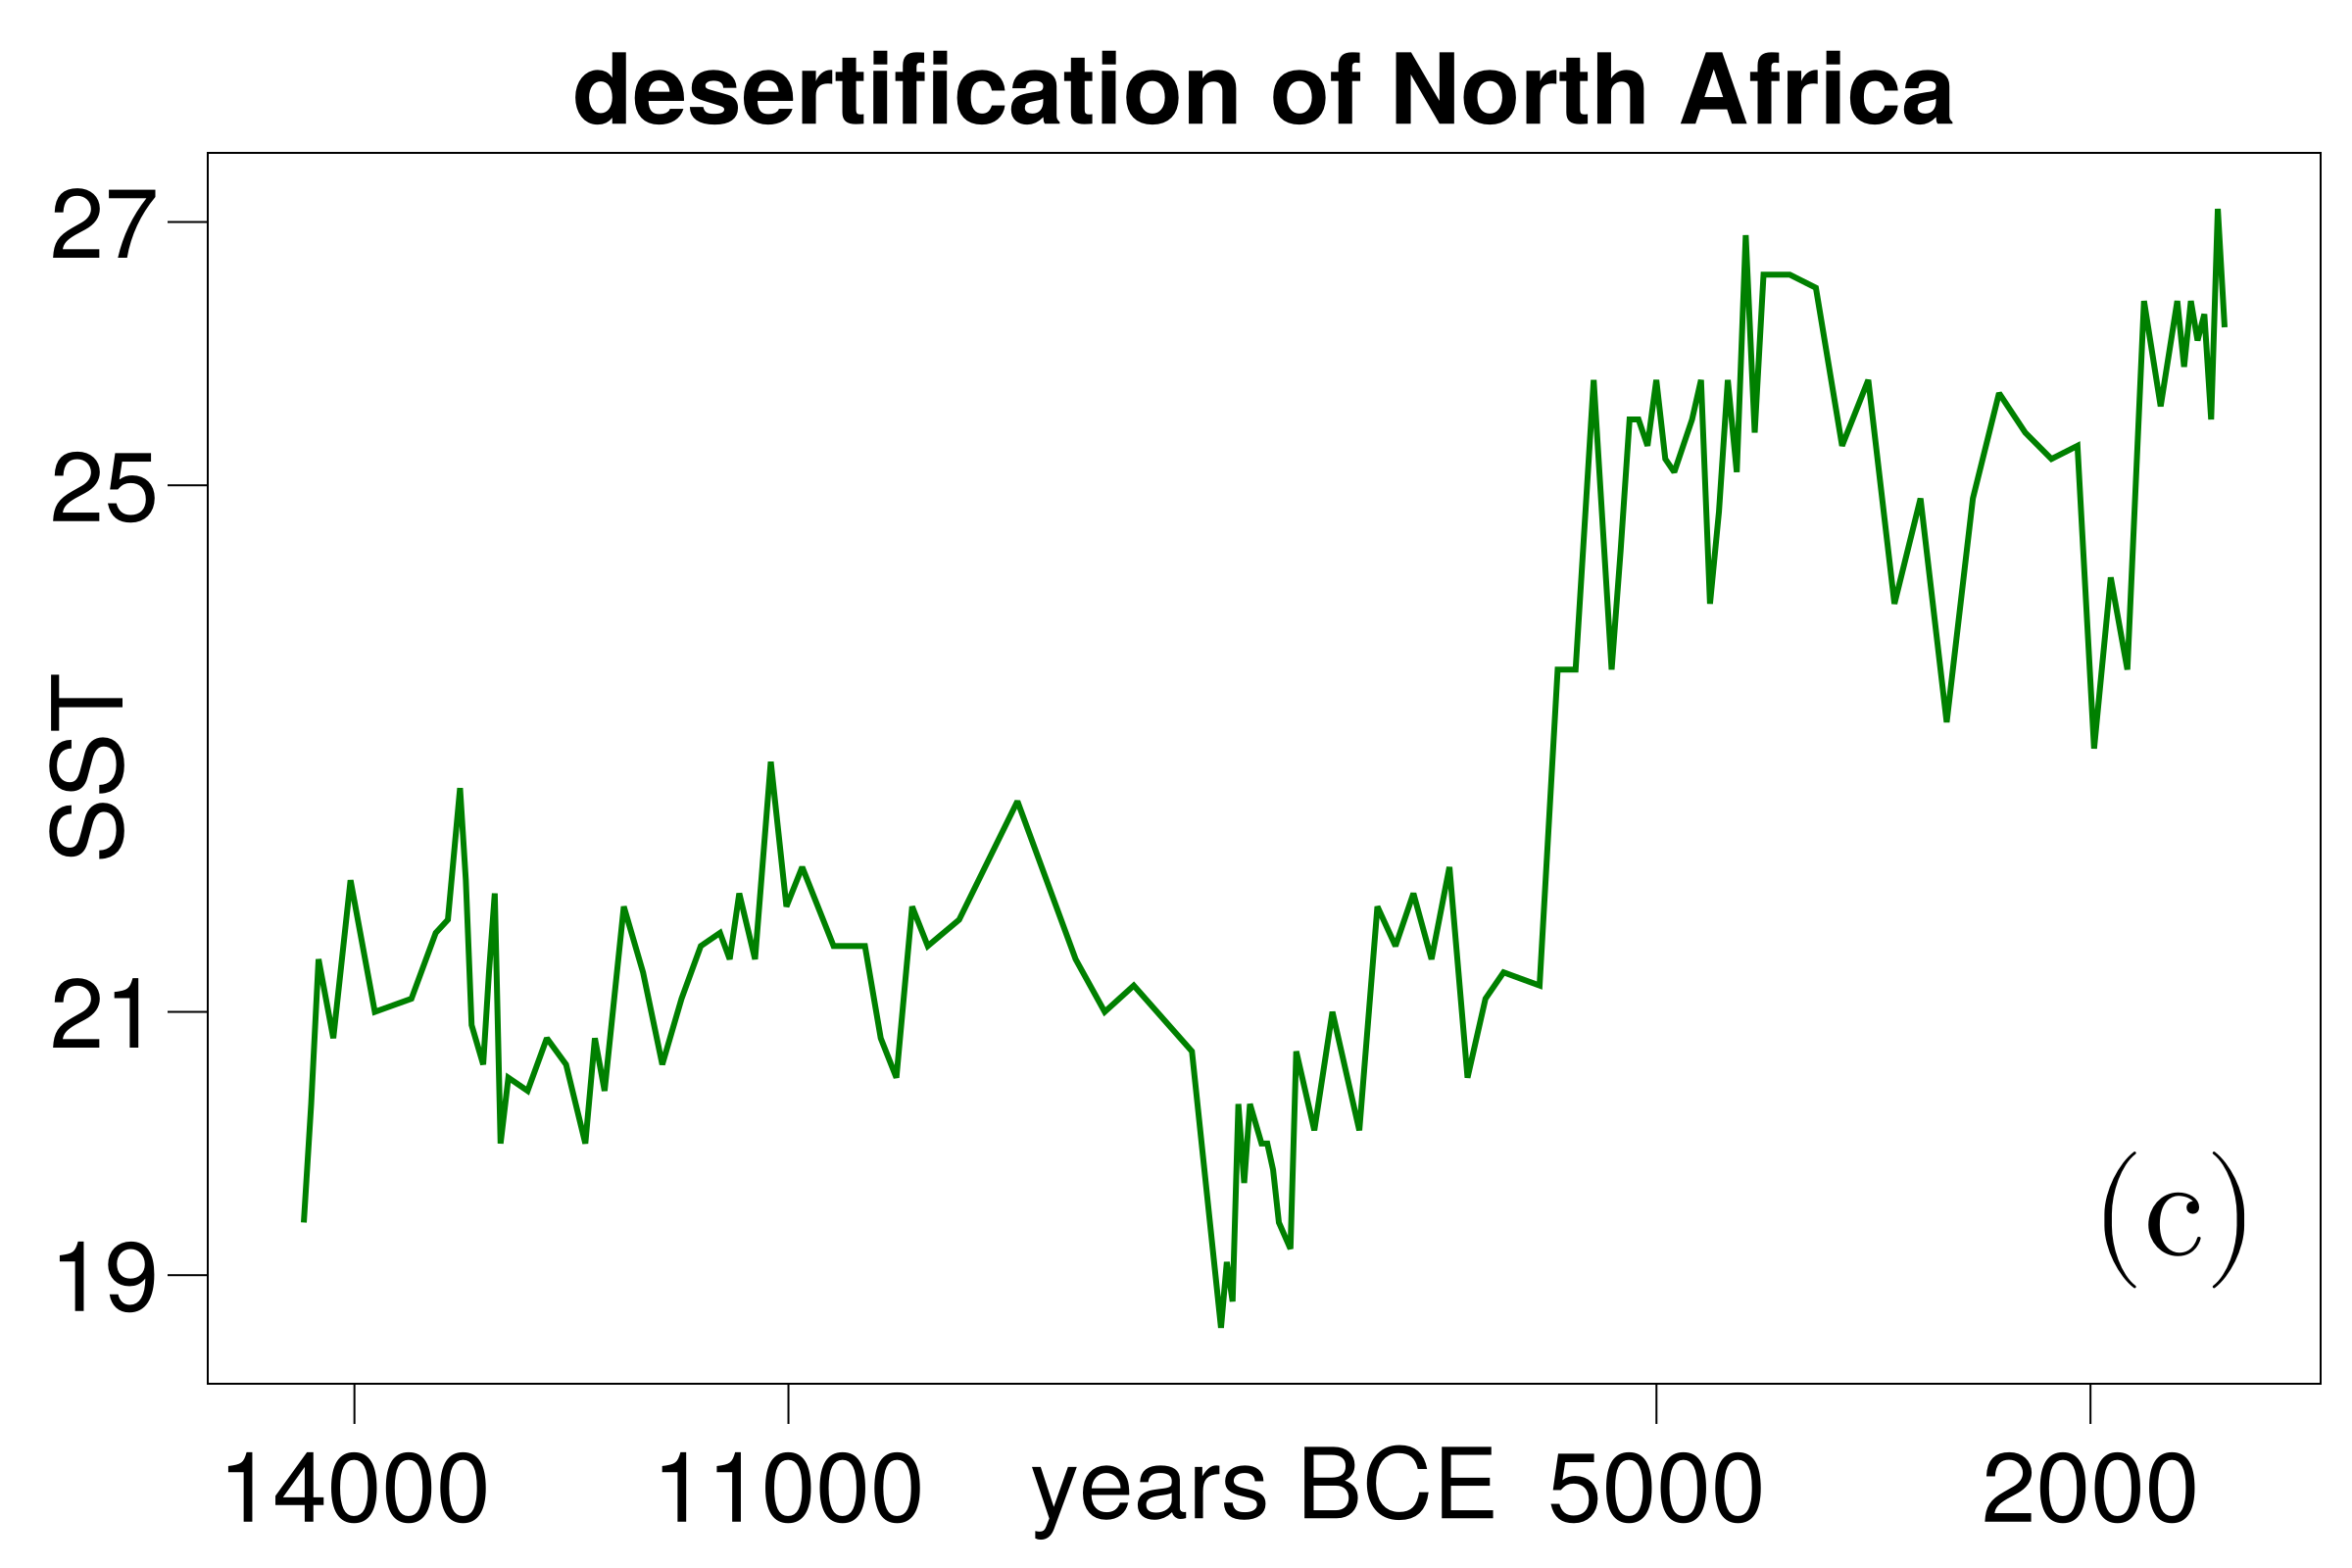
\includegraphics[keepaspectratio, width = \linewidth]{../figures/fig1.1.3.png}
        \label{fig1.1.3}
    \end{subfigure}


    \begin{subfigure}[b]{0.325\textwidth}
        \centering 
        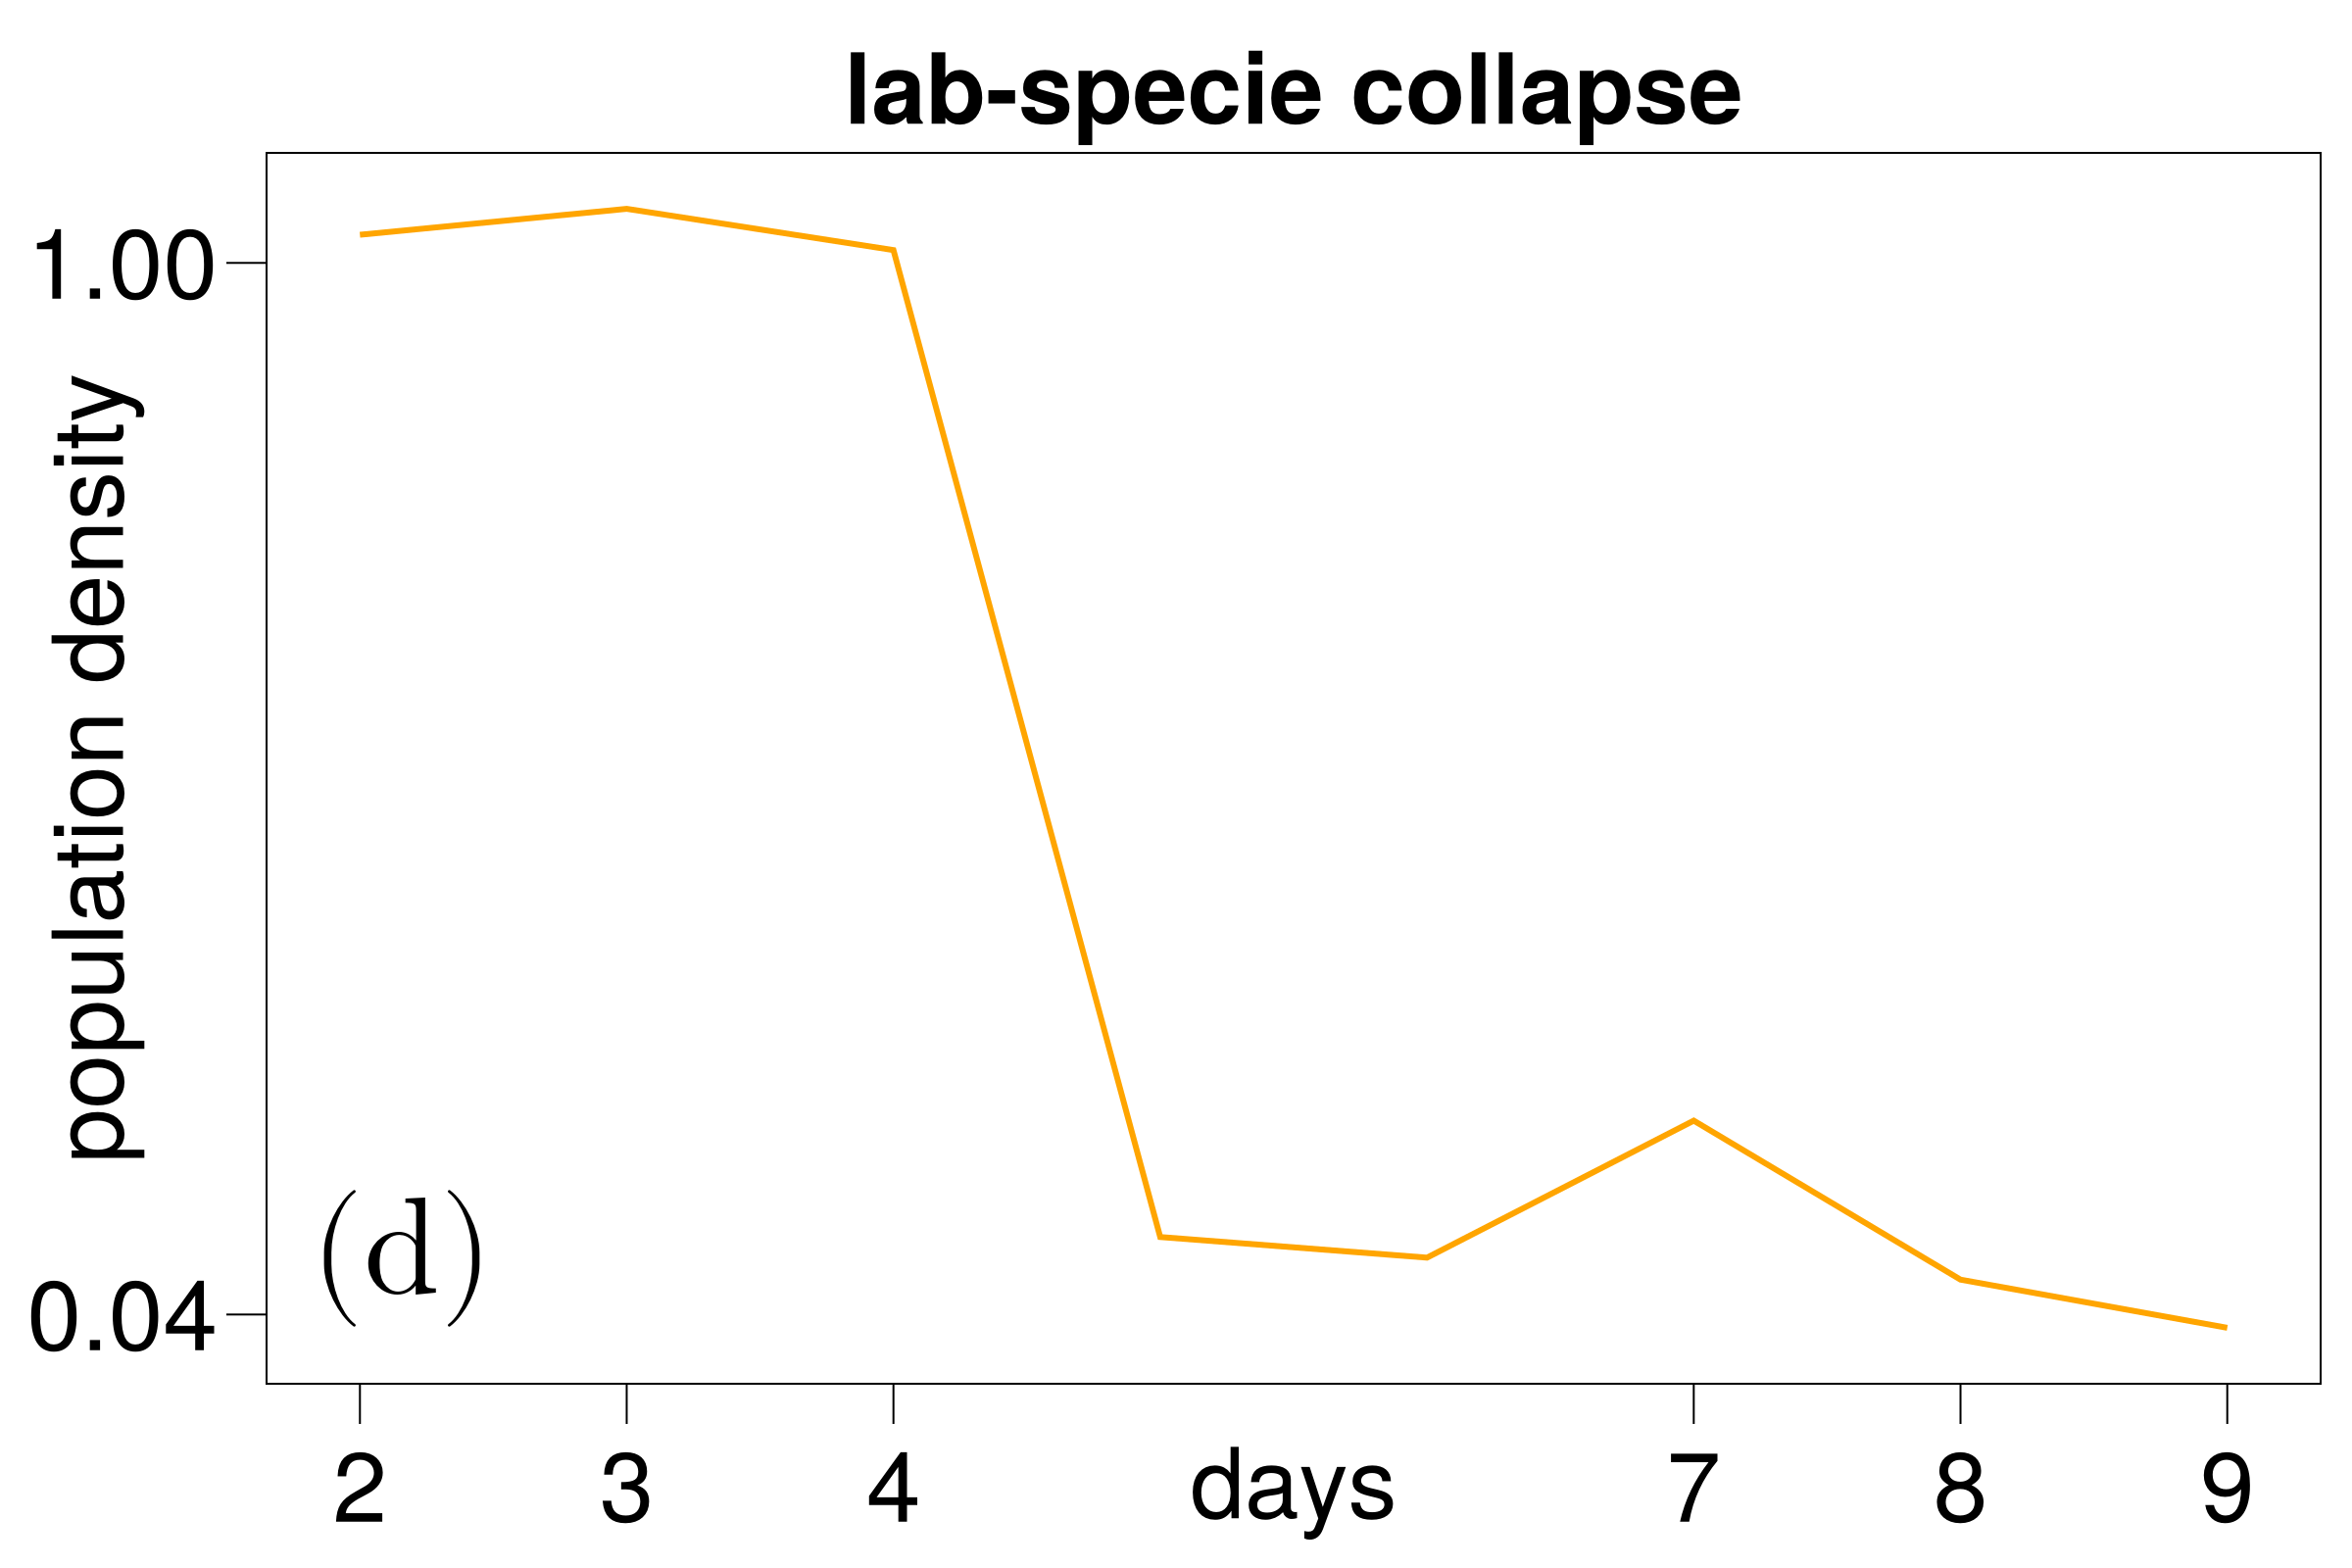
\includegraphics[keepaspectratio, width = \linewidth]{../figures/fig1.1.4.png}
        \label{fig1.1.4}
    \end{subfigure}
    \hfill
    \begin{subfigure}[b]{0.325\textwidth}
        \centering 
        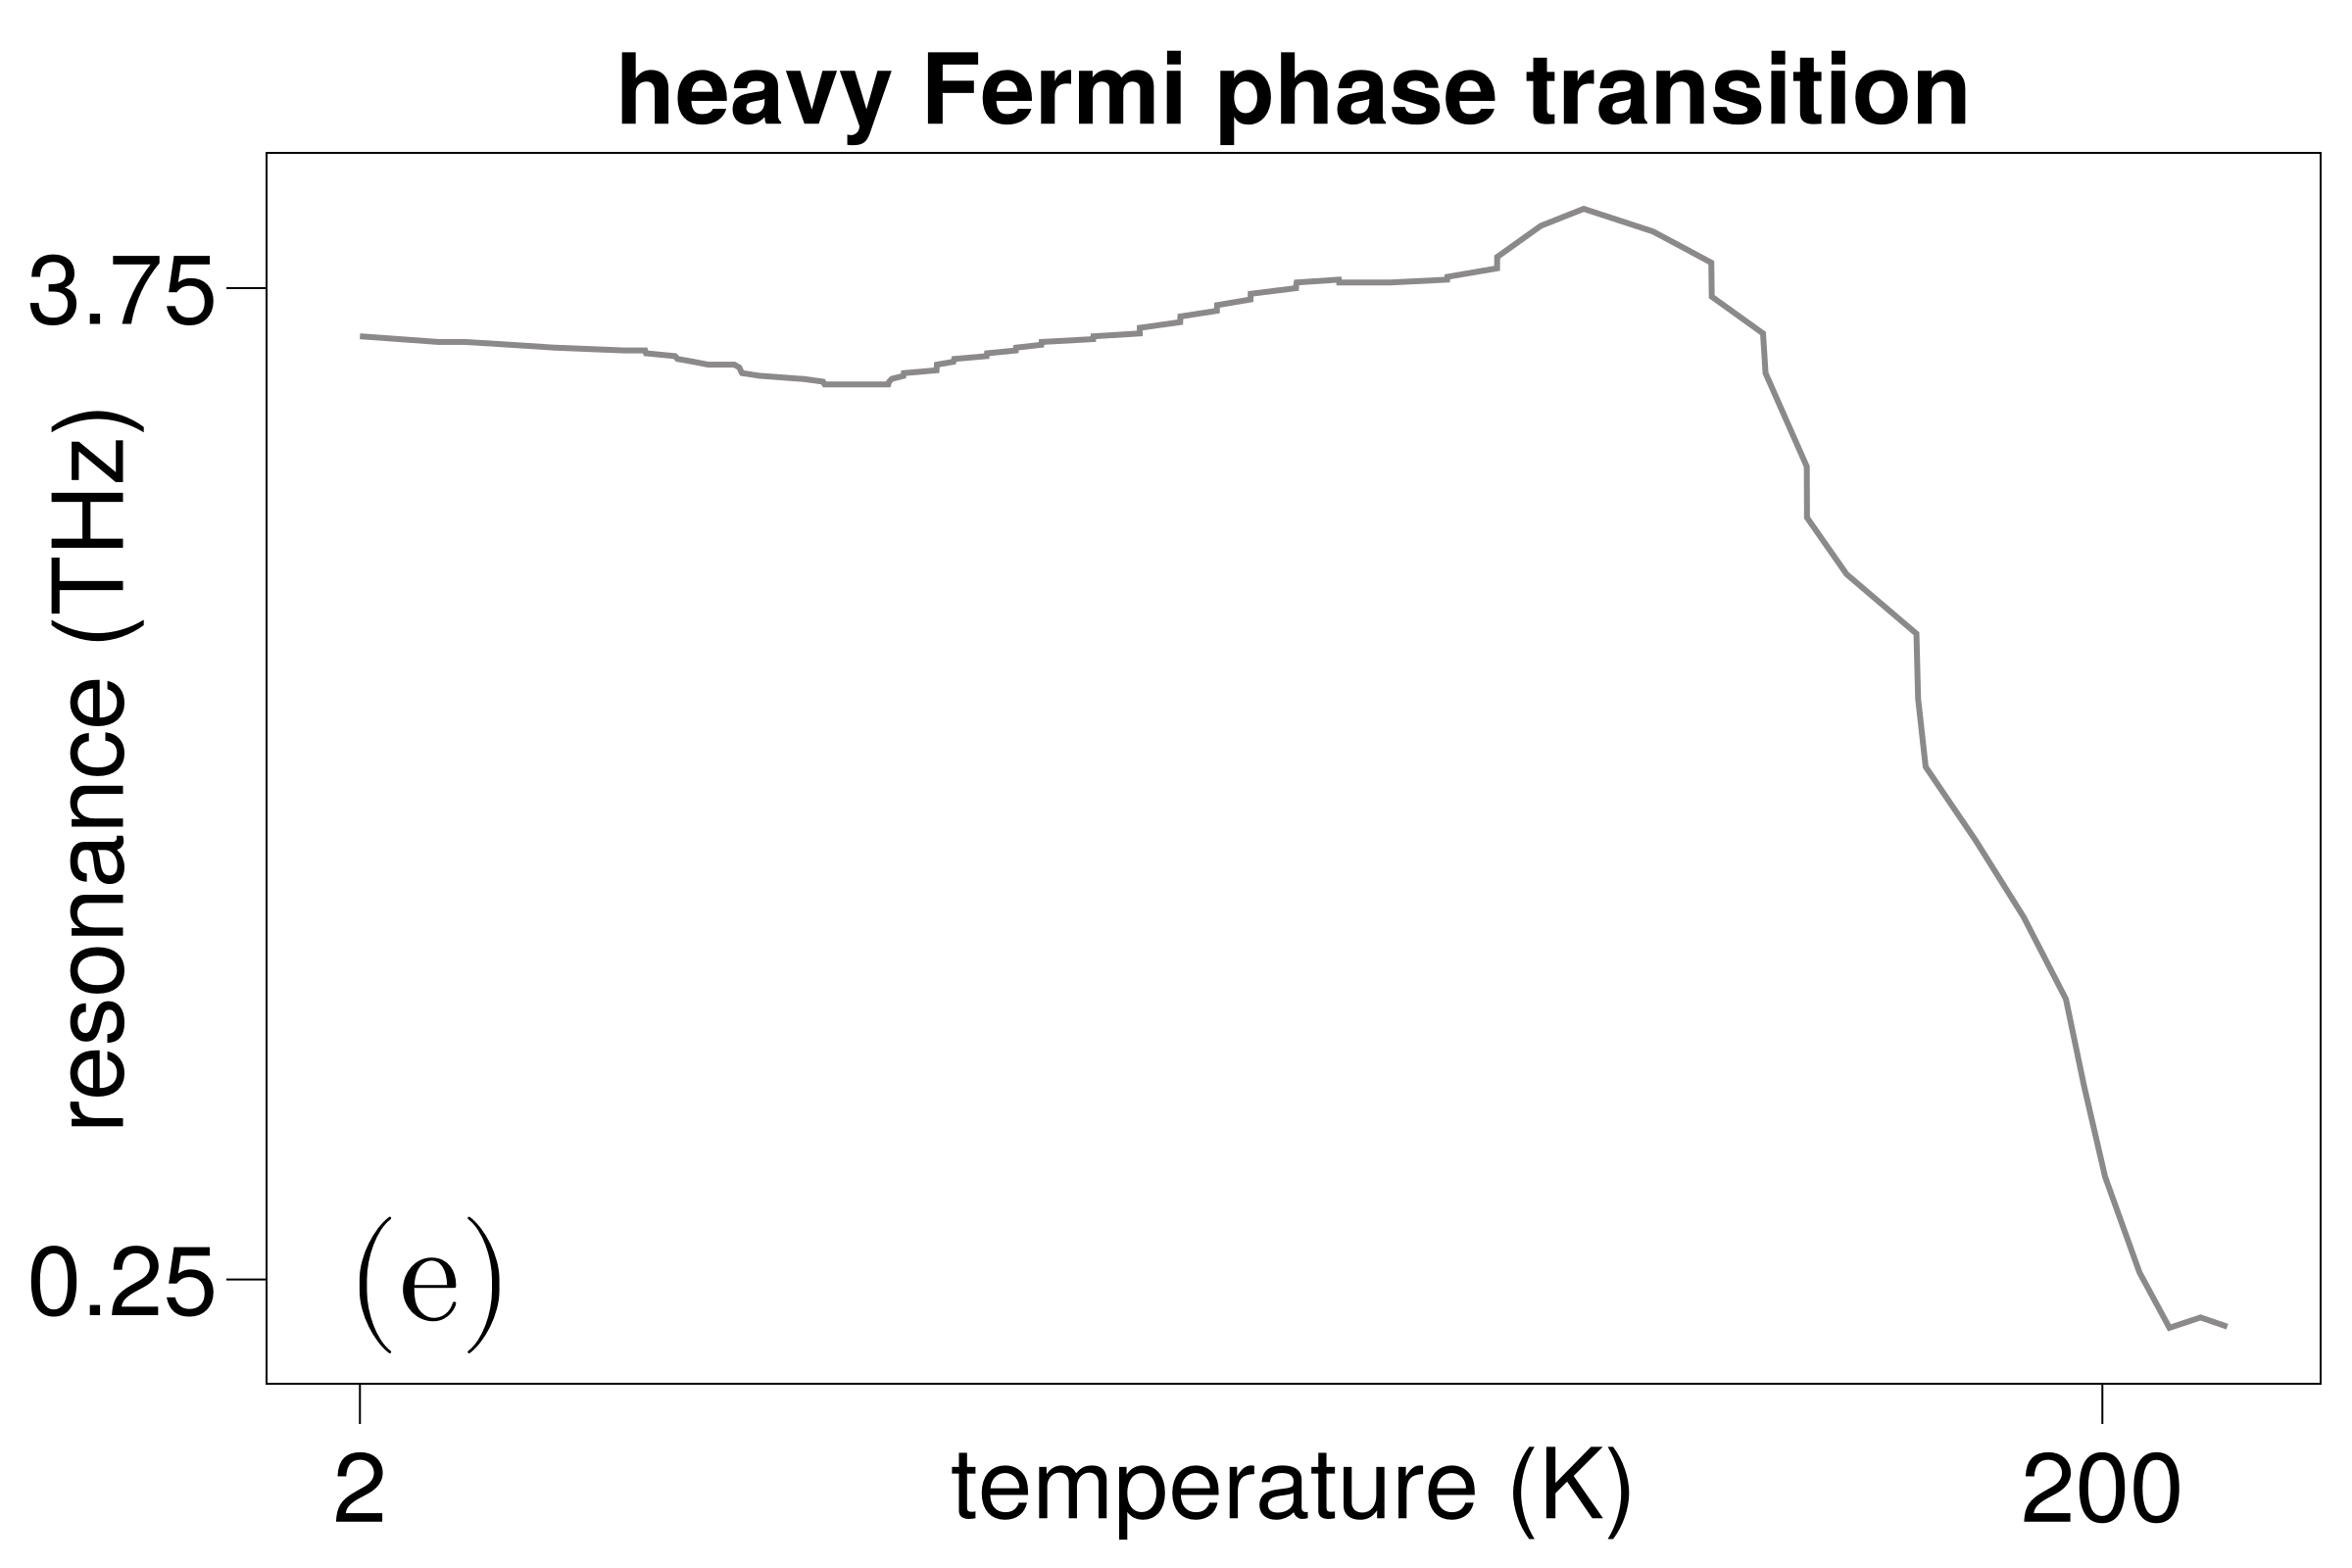
\includegraphics[keepaspectratio, width = \linewidth]{../figures/fig1.1.5.png}
        \label{fig1.1.5}
    \end{subfigure}
    \hfill
    \begin{subfigure}[b]{0.325\textwidth}
        \centering 
        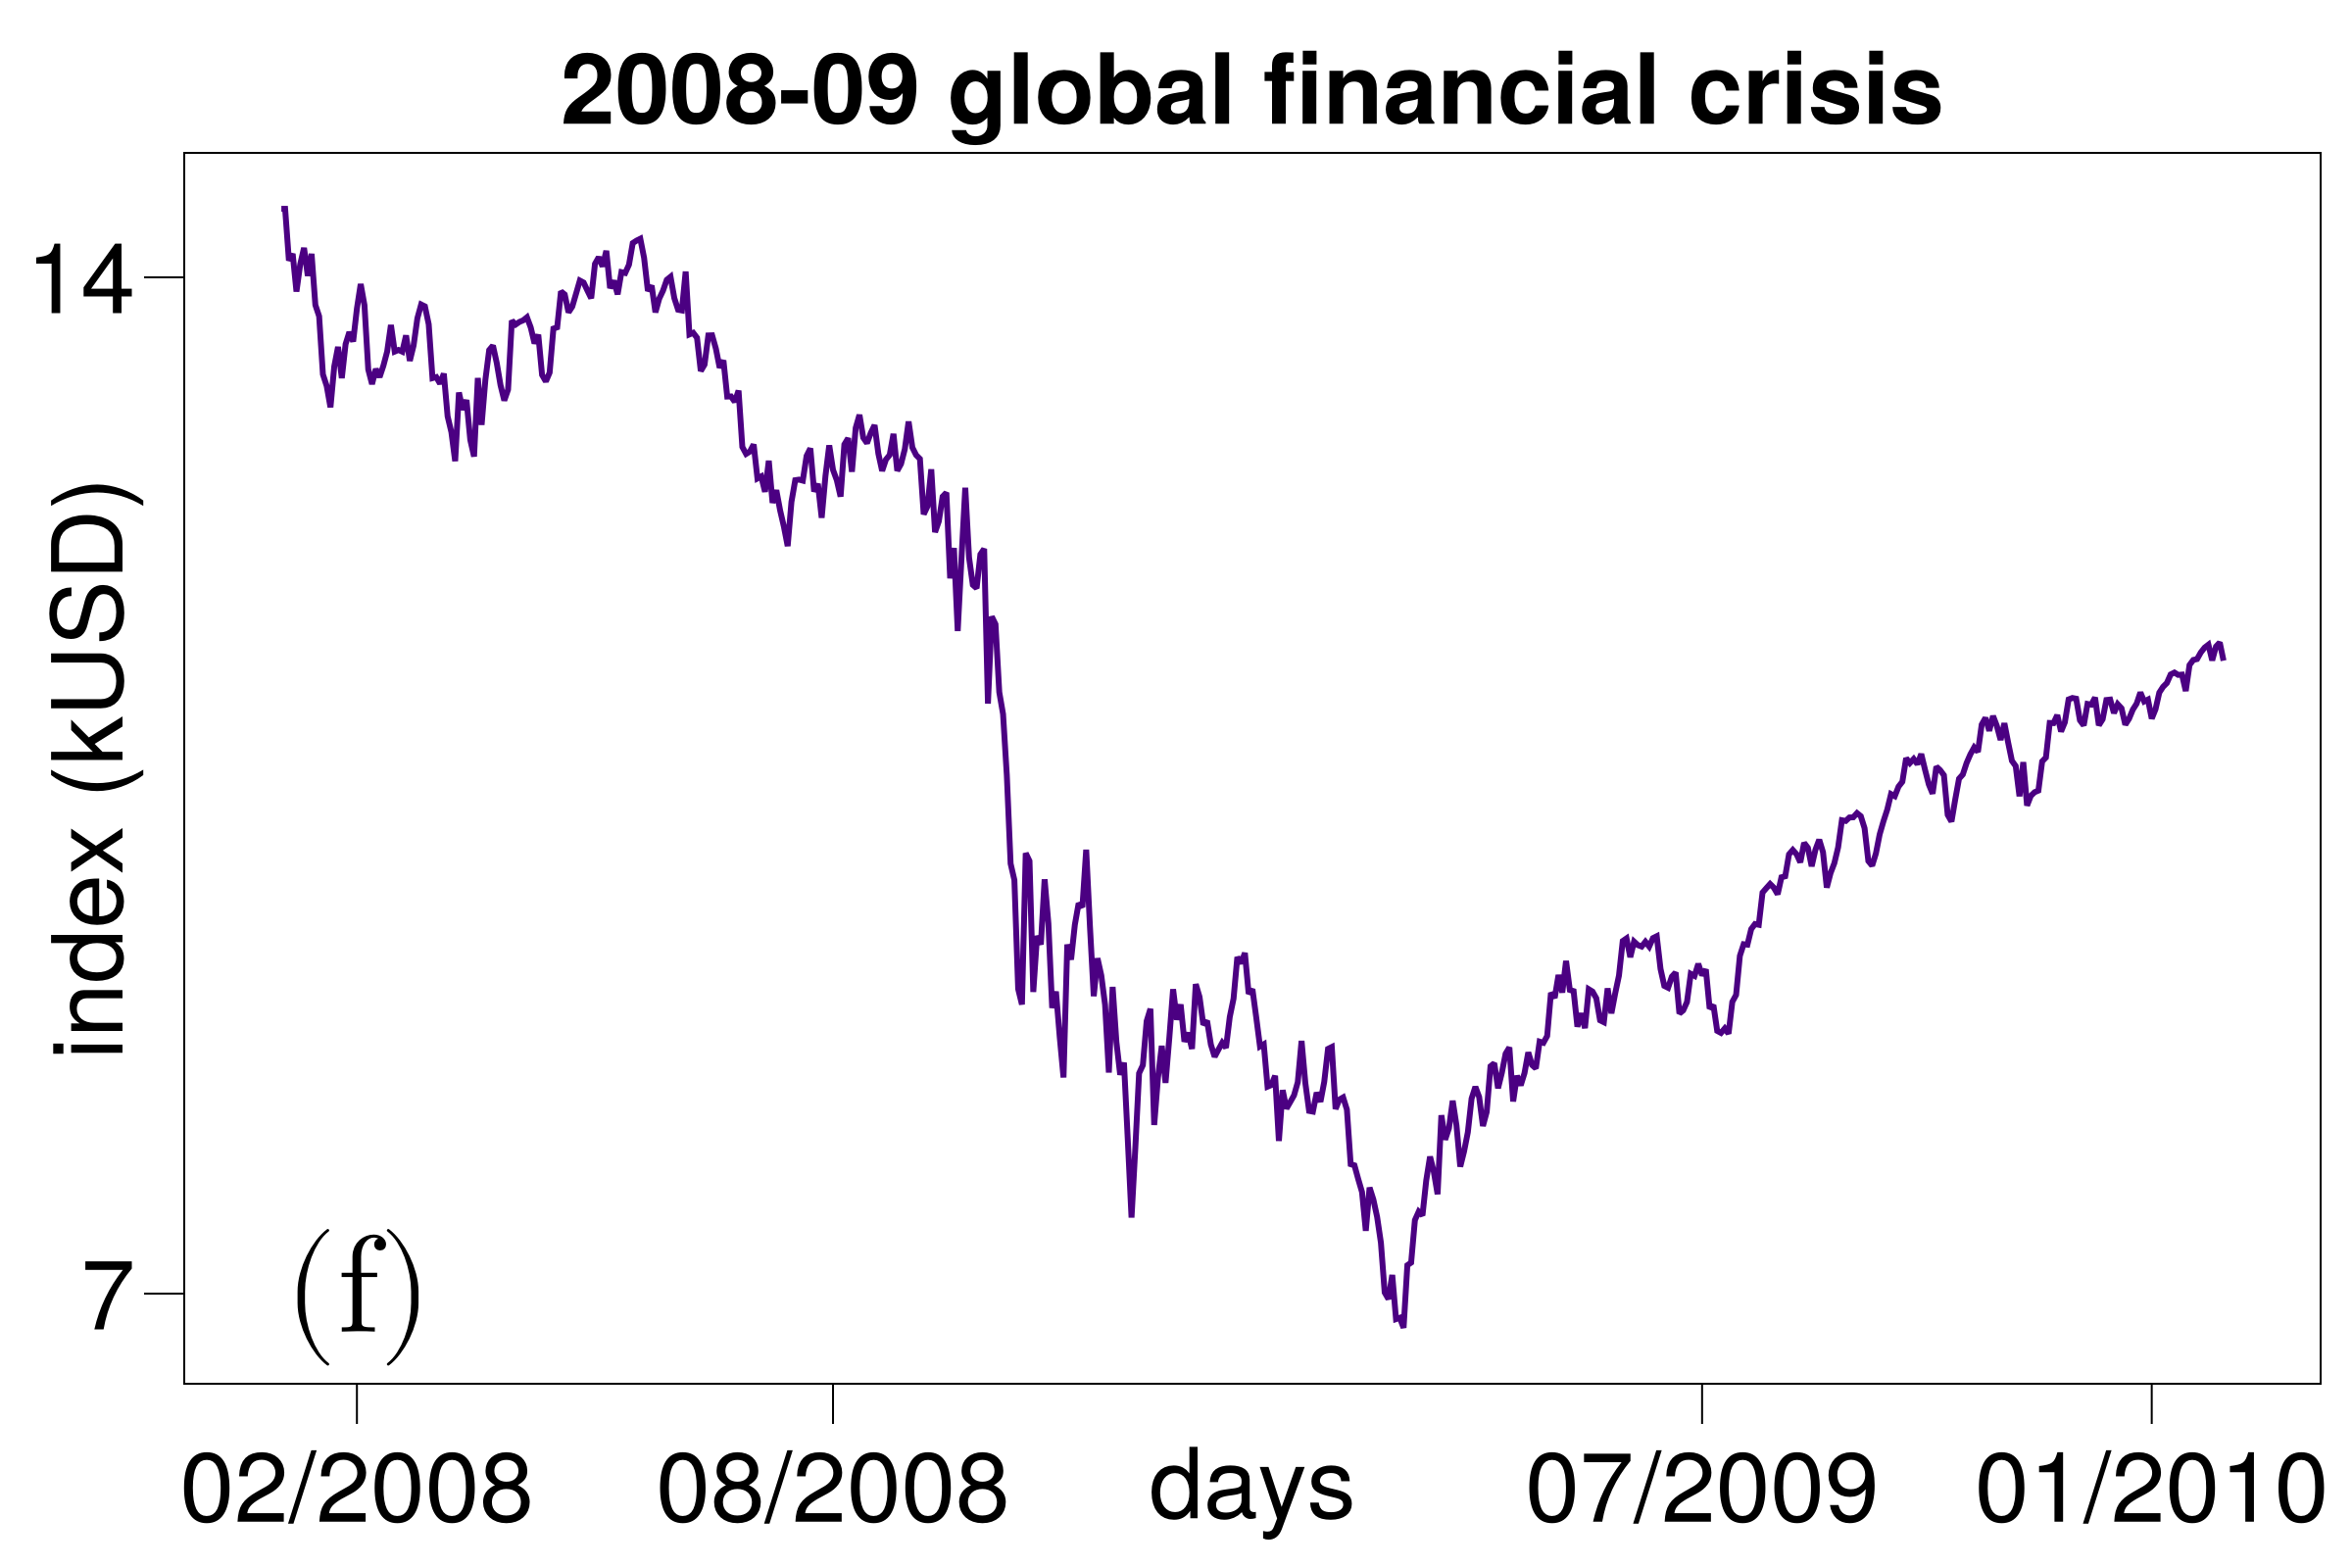
\includegraphics[keepaspectratio, width = \linewidth]{../figures/fig1.1.6.png}
        \label{fig1.1.6}
    \end{subfigure}
    \caption{Examples of real-world timeseries exhibiting a sudden regime shift (tipping event): (a) transition from Greenhouse to Icehouse Earth measured by calcium carbonate (CaCO$_3$) concentration in sediments of the tropical Pacific; (b) end of the last glacial period (LGP), colloquially referred to as the last ice age, detected as a transition of Deuterium ($2$H) concentrations in the ice core of Vostok, Antarctica; (c) abrupt end of the African humid period and onset of desertification from mean sea surface temperature (SST) measured in oceanic drilled holes off the cost of North-East Africa; (d) population collapse of a lab-grown ecosystem of budding yeast; (e) quantum phase transition from antiferromagnetic to heavy Fermi liquid of YbRh$_2$Si$_2$ measured as fermionic breakdown causing an abrupt decay of the resonant (spectroscopy) frequency; (f) global financial crisis caused by the collapse of subprime mortgages reflected by the Standard and Poor's 500 (S\&P 500) stock market index.
    Information about the sources of these study and the data points for the timeseries is provided in the Supplementary material.}
    \label{fig1.1}
\end{figure}
\end{document}
